\documentclass[tikz,border=2mm]{standalone}
\usepackage{amssymb}
\usepackage{amsmath}
\usepackage{pgfplots}
\usetikzlibrary[arrows.meta]
\usetikzlibrary{positioning, shapes, calc, backgrounds}
\usetikzlibrary{calc,trees,positioning,arrows,fit,shapes,calc}
\tikzset{set/.style={draw,circle,inner sep=0pt,align=center}}
\tikzset{line/.style = {draw,thick, shorten >=-2pt, shorten <=-2pt}}
\tikzset{tick/.style={draw, minimum width=0pt, minimum height=2pt, inner sep=0pt, label=below:$#1$},tick/.default={}}

\begin{document}
	
	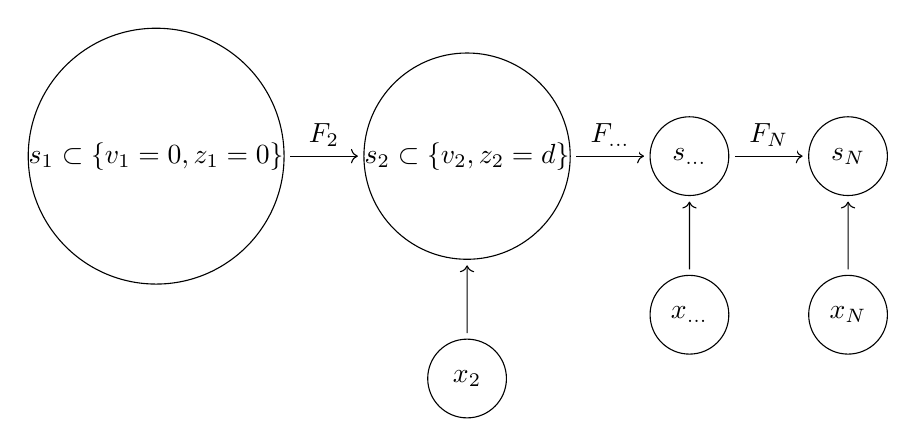
\begin{tikzpicture}[scale=0.3]
		% Draw grid
		\node[set, minimum size=2cm] (s1) {$s_1 \subset \{v_1 = 0, z_1= 0\}$};
		\node[set, minimum size=1cm, right = of s1] (s2) {$s_2\subset \{v_2, z_2 = d\}$};
		\node[set, minimum size=1cm, below = of s2] (x2) {$x_2$};
		\node[set, minimum size=1cm, right = of s2] (sd) {$s_{\dots}$};
		\node[set, minimum size=1cm, below = of sd] (xd) {$x_{\dots}$};
		\node[set, minimum size=1cm, right = of sd] (sn) {$s_{N}$};
		\node[set, minimum size=1cm, below = of sn] (xn) {$x_{N}$};
		% Draw an arrow from set A to set B
		\draw[->,shorten <=2pt,shorten >=2] (s1) -- node[above, align=center, fill = white] {$F_2$} (s2) ;
		\draw[->,shorten <=2pt,shorten >=2] (x2) -- (s2);
		\draw[->,shorten <=2pt,shorten >=2] (s2) -- node[above, align=center, fill = white] {$F_{\dots}$} (sd);
		\draw[->,shorten <=2pt,shorten >=2] (xd) -- (sd);
		\draw[->,shorten <=2pt,shorten >=2] (sd) -- node[above, align=center, fill = white] {$F_N$} (sn);
		\draw[->,shorten <=2pt,shorten >=2] (xn) -- (sn);
	\end{tikzpicture}
	
\end{document}
